
\documentclass[a4paper,11pt]{article}
\usepackage[a4paper, margin=8em]{geometry}

% usa i pacchetti per la scrittura in italiano
\usepackage[french,italian]{babel}
\usepackage[T1]{fontenc}
\usepackage[utf8]{inputenc}
\frenchspacing 

% usa i pacchetti per la formattazione matematica
\usepackage{amsmath, amssymb, amsthm, amsfonts}

% usa altri pacchetti
\usepackage{gensymb}
\usepackage{hyperref}
\usepackage{standalone}

\usepackage{colortbl}

\usepackage{xstring}
\usepackage{karnaugh-map}

% imposta il titolo
\title{Appunti Calcolatori Elettronici}
\author{Luca Seggiani}
\date{2025}

% imposta lo stile
% usa helvetica
\usepackage[scaled]{helvet}
% usa palatino
\usepackage{palatino}
% usa un font monospazio guardabile
\usepackage{lmodern}

\renewcommand{\rmdefault}{ppl}
\renewcommand{\sfdefault}{phv}
\renewcommand{\ttdefault}{lmtt}

% circuiti
\usepackage{circuitikz}
\usetikzlibrary{babel}

% testo cerchiato
\newcommand*\circled[1]{\tikz[baseline=(char.base)]{
            \node[shape=circle,draw,inner sep=2pt] (char) {#1};}}

% disponi il titolo
\makeatletter
\renewcommand{\maketitle} {
	\begin{center} 
		\begin{minipage}[t]{.8\textwidth}
			\textsf{\huge\bfseries \@title} 
		\end{minipage}%
		\begin{minipage}[t]{.2\textwidth}
			\raggedleft \vspace{-1.65em}
			\textsf{\small \@author} \vfill
			\textsf{\small \@date}
		\end{minipage}
		\par
	\end{center}

	\thispagestyle{empty}
	\pagestyle{fancy}
}
\makeatother

% disponi teoremi
\usepackage{tcolorbox}
\newtcolorbox[auto counter, number within=section]{theorem}[2][]{%
	colback=blue!10, 
	colframe=blue!40!black, 
	sharp corners=northwest,
	fonttitle=\sffamily\bfseries, 
	title=Teorema~\thetcbcounter: #2, 
	#1
}

% disponi definizioni
\newtcolorbox[auto counter, number within=section]{definition}[2][]{%
	colback=red!10,
	colframe=red!40!black,
	sharp corners=northwest,
	fonttitle=\sffamily\bfseries,
	title=Definizione~\thetcbcounter: #2,
	#1
}

% disponi codice
\usepackage{listings}
\usepackage[table]{xcolor}

\definecolor{codegreen}{rgb}{0,0.6,0}
\definecolor{codegray}{rgb}{0.5,0.5,0.5}
\definecolor{codepurple}{rgb}{0.58,0,0.82}
\definecolor{backcolour}{rgb}{0.95,0.95,0.92}

\lstdefinestyle{codestyle}{
		backgroundcolor=\color{black!5}, 
		commentstyle=\color{codegreen},
		keywordstyle=\bfseries\color{magenta},
		numberstyle=\sffamily\tiny\color{black!60},
		stringstyle=\color{green!50!black},
		basicstyle=\ttfamily\footnotesize,
		breakatwhitespace=false,         
		breaklines=true,                 
		captionpos=b,                    
		keepspaces=true,                 
		numbers=left,                    
		numbersep=5pt,                  
		showspaces=false,                
		showstringspaces=false,
		showtabs=false,                  
		tabsize=2
}

\lstdefinestyle{shellstyle}{
		backgroundcolor=\color{black!5}, 
		basicstyle=\ttfamily\footnotesize\color{black}, 
		commentstyle=\color{black}, 
		keywordstyle=\color{black},
		numberstyle=\color{black!5},
		stringstyle=\color{black}, 
		showspaces=false,
		showstringspaces=false, 
		showtabs=false, 
		tabsize=2, 
		numbers=none, 
		breaklines=true
}


\lstdefinelanguage{assembler}{ 
  keywords={AAA, AAD, AAM, AAS, ADC, ADCB, ADCW, ADCL, ADD, ADDB, ADDW, ADDL, AND, ANDB, ANDW, ANDL,
        ARPL, BOUND, BSF, BSFL, BSFW, BSR, BSRL, BSRW, BSWAP, BT, BTC, BTCB, BTCW, BTCL, BTR, 
        BTRB, BTRW, BTRL, BTS, BTSB, BTSW, BTSL, CALL, CBW, CDQ, CLC, CLD, CLI, CLTS, CMC, CMP,
        CMPB, CMPW, CMPL, CMPS, CMPSB, CMPSD, CMPSW, CMPXCHG, CMPXCHGB, CMPXCHGW, CMPXCHGL,
        CMPXCHG8B, CPUID, CWDE, DAA, DAS, DEC, DECB, DECW, DECL, DIV, DIVB, DIVW, DIVL, ENTER,
        HLT, IDIV, IDIVB, IDIVW, IDIVL, IMUL, IMULB, IMULW, IMULL, IN, INB, INW, INL, INC, INCB,
        INCW, INCL, INS, INSB, INSD, INSW, INT, INT3, INTO, INVD, INVLPG, IRET, IRETD, JA, JAE,
        JB, JBE, JC, JCXZ, JE, JECXZ, JG, JGE, JL, JLE, JMP, JNA, JNAE, JNB, JNBE, JNC, JNE, JNG,
        JNGE, JNL, JNLE, JNO, JNP, JNS, JNZ, JO, JP, JPE, JPO, JS, JZ, LAHF, LAR, LCALL, LDS,
        LEA, LEAVE, LES, LFS, LGDT, LGS, LIDT, LMSW, LOCK, LODSB, LODSD, LODSW, LOOP, LOOPE,
        LOOPNE, LSL, LSS, LTR, MOV, MOVB, MOVW, MOVL, MOVSB, MOVSD, MOVSW, MOVSX, MOVSXB,
        MOVSXW, MOVSXL, MOVZX, MOVZXB, MOVZXW, MOVZXL, MUL, MULB, MULW, MULL, NEG, NEGB, NEGW,
        NEGL, NOP, NOT, NOTB, NOTW, NOTL, OR, ORB, ORW, ORL, OUT, OUTB, OUTW, OUTL, OUTSB, OUTSD,
        OUTSW, POP, POPL, POPW, POPB, POPA, POPAD, POPF, POPFD, PUSH, PUSHL, PUSHW, PUSHB, PUSHA, 
				PUSHAD, PUSHF, PUSHFD, RCL, RCLB, RCLW, MOVSL, MOVSB, MOVSW, STOSL, STOSB, STOSW, LODSB, LODSW,
				LODSL, INSB, INSW, INSL, OUTSB, OUTSL, OUTSW
        RCLL, RCR, RCRB, RCRW, RCRL, RDMSR, RDPMC, RDTSC, REP, REPE, REPNE, RET, ROL, ROLB, ROLW,
        ROLL, ROR, RORB, RORW, RORL, SAHF, SAL, SALB, SALW, SALL, SAR, SARB, SARW, SARL, SBB,
        SBBB, SBBW, SBBL, SCASB, SCASD, SCASW, SETA, SETAE, SETB, SETBE, SETC, SETE, SETG, SETGE,
        SETL, SETLE, SETNA, SETNAE, SETNB, SETNBE, SETNC, SETNE, SETNG, SETNGE, SETNL, SETNLE,
        SETNO, SETNP, SETNS, SETNZ, SETO, SETP, SETPE, SETPO, SETS, SETZ, SGDT, SHL, SHLB, SHLW,
        SHLL, SHLD, SHR, SHRB, SHRW, SHRL, SHRD, SIDT, SLDT, SMSW, STC, STD, STI, STOSB, STOSD,
        STOSW, STR, SUB, SUBB, SUBW, SUBL, TEST, TESTB, TESTW, TESTL, VERR, VERW, WAIT, WBINVD,
        XADD, XADDB, XADDW, XADDL, XCHG, XCHGB, XCHGW, XCHGL, XLAT, XLATB, XOR, XORB, XORW, XORL},
  keywordstyle=\color{blue}\bfseries,
  ndkeywordstyle=\color{darkgray}\bfseries,
  identifierstyle=\color{black},
  sensitive=false,
  comment=[l]{\#},
  morecomment=[s]{/*}{*/},
  commentstyle=\color{purple}\ttfamily,
  stringstyle=\color{red}\ttfamily,
  morestring=[b]',
  morestring=[b]"
}

\lstset{language=assembler, style=codestyle}

% disponi sezioni
\usepackage{titlesec}

\titleformat{\section}
	{\sffamily\Large\bfseries} 
	{\thesection}{1em}{} 
\titleformat{\subsection}
	{\sffamily\large\bfseries}   
	{\thesubsection}{1em}{} 
\titleformat{\subsubsection}
	{\sffamily\normalsize\bfseries} 
	{\thesubsubsection}{1em}{}

% tikz
\usepackage{tikz}

% float
\usepackage{float}

% grafici
\usepackage{pgfplots}
\pgfplotsset{width=10cm,compat=1.9}

% disponi alberi
\usepackage{forest}

\forestset{
	rectstyle/.style={
		for tree={rectangle,draw,font=\large\sffamily}
	},
	roundstyle/.style={
		for tree={circle,draw,font=\large}
	}
}

% disponi algoritmi
\usepackage{algorithm}
\usepackage{algorithmic}
\makeatletter
\renewcommand{\ALG@name}{Algoritmo}
\makeatother

% disponi numeri di pagina
\usepackage{fancyhdr}
\fancyhf{} 
\fancyfoot[L]{\sffamily{\thepage}}

\makeatletter
\fancyhead[L]{\raisebox{1ex}[0pt][0pt]{\sffamily{\@title \ \@date}}} 
\fancyhead[R]{\raisebox{1ex}[0pt][0pt]{\sffamily{\@author}}}
\makeatother

\begin{document}
% sezione (data)
\section{Lezione del 09-05-25}

% stili pagina
\thispagestyle{empty}
\pagestyle{fancy}

% testo
Riprendiamo il discorso sull'architettura del processore.
Possiamo fare un riassunto dell'architettura descritta finora:
\begin{center}
	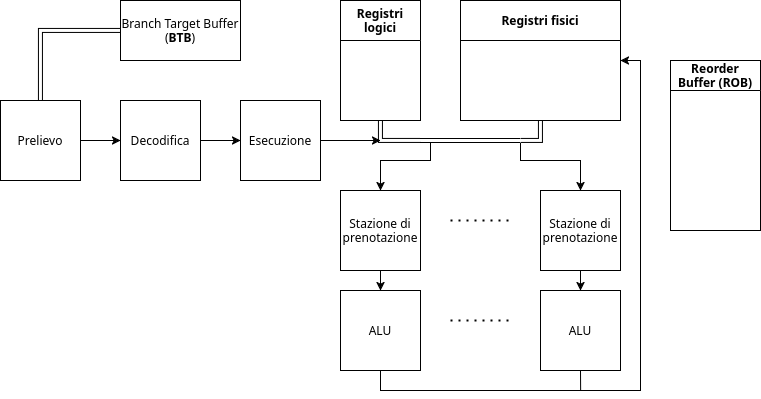
\includegraphics[scale=.55]{../figures/arch1.png}
\end{center}

Abbiamo quindi che le istruzioni provengono dal Branch Target Buffer, \textbf{BTB}, dalle quali vengono poste in una componente di \textbf{prelievo} e una di \textbf{decodifica}.

Da qui i poi le istruzioni passano per le stazioni di prenotazione, che poi le inviano alle relative ALU, sulla base delle tabelle associate ai registri fisici.

In fine, in fondo a questo meccanismo si trova il Reorder Buffer, \textbf{ROB}, che contiene le istruzioni terminate ma non ancora scritte e permette l'esecuzione speculativa.
Il significato del Reorder Buffer è sostanzialmente quello di realizzare un'ulteriore smistamento delle istruzioni a termine della loro esecuzione, che permette o meno il loro write back nei registri (che sappiamo coi registri ridenominati significa semplicemente aggiornare i registri logici) solo sotto le condizioni dell'esecuzione speculativa.

\subsubsection{Istruzioni LOAD e STORE}
L'esecuzione speculativa vista presenta problemi per quanto riguarda le istruzioni \lstinline|LOAD| e \lstinline|STORE|.

Prendiamo ad esempio il framento di codice:
\begin{lstlisting}	
	cmp $1000, %rbx
	jae fine
	mov off(%rbx), %rax

fine:
\end{lstlisting}

Qui la scrittura va eseguita solo se \lstinline|%rbx| contiene un valore inferiore a mille.
Per le regole dei salti in avanti, il salto in \lstinline|jae fine| si da per non fatto, e quindi il BTB fornisce l'istruzione successiva, cioè quella di accesso in memoria (che verrebbe tradotta in una \lstinline|load|). # capito 0, per le store come fa?

\subsubsection{Istruzioni IN e OUT}
Infine, una nota va fatta sulle istruzioni di I/O \lstinline|in| e \lstinline|out|: queste infatti hanno conseguenze su dispositivi esterni al processore per cui non ne si può fare l'esecuzione parallela o speculativa.

In fase di emissione di istruzioni di I/o, quindi, il processore si aspetta che tutte le istruzioni attualmente in esecuzione siano state eseguite, e solo dopo procede con l'emissione. # e poi?

\subsection{Vulnerabilità Meltdown e Spectre}
\textbf{Meltdown} e \textbf{Spectre} sono state vulnerabilità dell'architettura Intel x86, scoperte nel 2017, che permettevano di superare le limitazioni normalmente imposte al codice in esecuzione in modalità utente.

Abbiamo detto che il programma dovrebbe poter ignorare ciò che accade nel processore a livello \textbf{microarchitetturale}, cioè che tutte le operazioni che l'architettura descritta finora compie ai fini di ottimizzare l'esecuzione devono risultare \textbf{invisibili} al programma.

Ciò che queste vulnerabilità hanno rivelato è che lo stato microarchitetturale, invece, non è veramente invisibile.

\subsubsection{Meltdown}
Ad esempio, per quanto riguarda la cache, abbiamo che si può in qualche modo capire se qualcosa è scritto in cache: bastera invalidare una cacheline, far eseguire il processo che vogliamo studiare, e quindi tentare un'accesso alla stessa cacheline: valutando il tempo necessario all'accesso (e magari facendo una media statistica) si potrà capira se quella cacheline è piena oppure no.

Questa era l'approccio adottato dalla vulnerabilità Meltdown.
\begin{lstlisting}	
togli_cacheline

mov indirizzo_vietato, %al # qui il programma muore
# da qui in poi si esegue in speculativa
shl $12, %al
mov vettore (%rax), %rbx

# questo si mette nell'handler del segmentation fault
controlla_cacheline
\end{lstlisting}

L'istruzione illegale \lstinline|mov indirizzo_vietato, %al| causerà chiaramente l'arresto del programma, ma le due istruzioni successive verranno comunque eseguite dal processore in modalità speculativa, prima che si manifesti il fault.

La \lstinline|controlla_cacheline|, invece, viene eseguita comunque attraverso una ridefinizione dell'handler di segmentation fault.

A questo punto, si ha quindi che l'indirizzo letto in \lstinline|%al|, che il processo non sarebbe autorizzato a vedere, viene trasformato in un indice in un vettore, vettore il cui accesso si traduce nel riempimento di una cachline che rileviamo in \lstinline|controlla_cacheline|.

Iterando questo processo su tutta la memoria kernel si riesce a ricostruirne una copia, e quindi effettivamente leggere tutta la memoria fisica.

Il problema oggi è stato risolto forzando l'invalidazione della cache ad ogni passaggio al kernel.

\subsubsection{Spectre}
La vulnerabilità Spectre si basa sulla natura stessa del branch prediction: l'utente può sfruttare la struttura del BTB, che abbiamo detto è effettivamente una cache senza controlli sulle collisioni, per "addestrare" il predittore di branch a fare scelte arbitrarie.

In questo modo si potrà in qualche modo "direzionare" l'esecuzione del kernel in luogo dei salti condizionali, e poi usando metodi come Meltdown capire che cosa il kernel ha fatto.

Anche questo problema si può risolvere invalidando una cache in fase di passaggio al kernel, e in particolare invalidando il BTB.

\end{document}
